\documentclass[10pt,a4paper]{report}
\usepackage[latin1]{inputenc}
\usepackage{amsmath}
\usepackage{amsfonts}
\usepackage{color}
\usepackage{amssymb}
\usepackage{graphicx}
\usepackage{fancyhdr}
\lhead{Introduction to \\ Computer Graphics}
\chead{Exercise number}
\rhead{Kevin Serrano, 204141 \\ Gianni Scarnera, 195899}
\pagestyle{fancy}
\author{Kevin Serrano, Gianni Scarnera}
\title{Exercise 3}
\date{24 October 2012}
\begin{document}
\maketitle

\section*{Part 3.2  Transformation and Translation}
First we have to calculate the dimension of the near plane. Given the angle in y-axis from the camera to the near plane and the distance of the near plan, we can calculate the distance of the $top,bottom,left,right$ from the center of the near plane.
\begin{figure}[h!]
\caption{Camera, near plane and far plane}
  \centering
    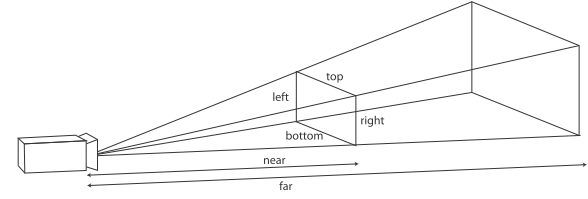
\includegraphics[width=0.7\textwidth]{plane.png}
\end{figure}
\begin{figure}[h!]
\caption{angle}
  \centering
    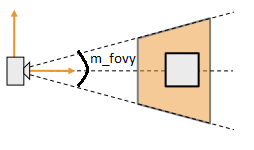
\includegraphics[width=0.5\textwidth]{angle.png}
\end{figure}
Then the half-height is given by trigonometric rule $$half\-height = nearPlane \cdot tan(m_{fovy}/2)$$ where m\_fovy is in degree. Then we can do a ration to figure out the half-width and then $$half\-width = half\-height \cdot Height/Width$$ where Height and Width are from the camera.
Then we can juste compute the $top,bottom,left,right$ as 	$bottom = -half\-height;
        top = half\-height;
        left = half\-width;
        right = -half\-width;$\\
Then the projection matrix is given in the course and is \[ \left( \begin{array}{cccc}
$$(2 \cdot n)/(r-l)$$ & 0 & $$(r+l)/(r-l)$$ & 0\\
0 & $$(2 \cdot n)/(t-b)$$ & $$(t+b)/(t-b)$$ & 0\\
0 & 0 & $$-(f+n)/(f-n)$$ & $$-(2nf)/(f-n)$$\\
0 & 0 & -1 & 0\end{array} \right)\] 
Then in the cube.vs file, we applied the transformation in this order to get the gl\_position :
$$gl_{Position} = (ProjectionMatrix * WorldCameraTransform * ModelWorldTransform) * gl_{Vertex};$$
\newpage

The translation matrix is given in the course: 
\[ \left( \begin{array}{cccc}
1 & 0 & 0 & t_x\\
0 & 1 & 0 & t_y\\
0 & 0 & 1 & t_z\\
0 & 0 & 0 & 1\end{array} \right)\] 
so we can return this matrix in $getTranslationMatrix()$

Now the difficulty to implement the $translateWorld()$ and $translateObject()$ functions is that we have to do the multiplication in correct order, because matrices multiplication isn't ever commutative as we've seen in lecture.
For $translateWorld()$, the translation must be applied after all previous matrices and it's the inverse for $translateObject()$, i.e :
for $translateWorld()$
$$m\_transformationMatrix = getTranslationMatrix(\_trans) \cdot m\_transformationMatrix;$$
and for $translateObject()$
$$m\_transformationMatrix = m\_transformationMatrix \cdot getTranslationMatrix(\_trans);$$
where $m\_transformationMatrix$ is the current transformation matrix.

\begin{figure}[h!]
\caption{Renderer the translation}
  \centering
    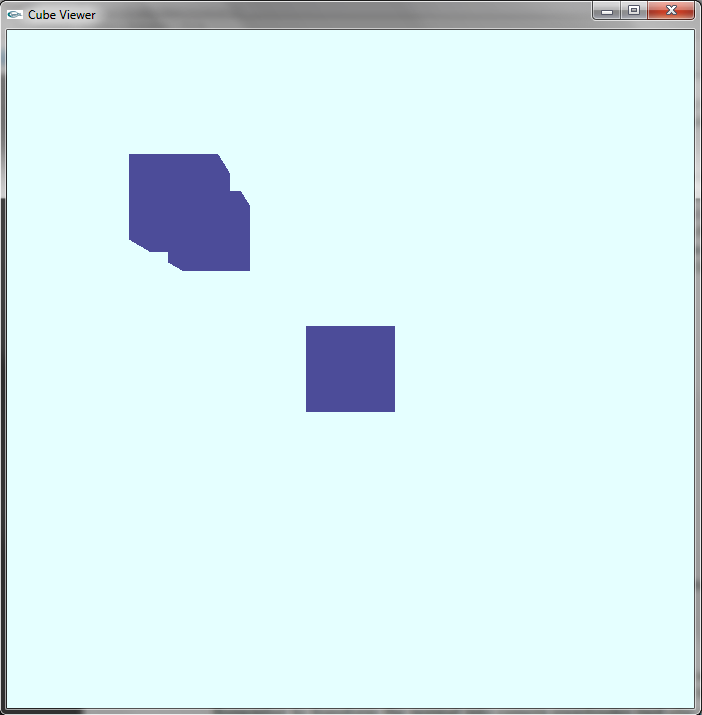
\includegraphics[width=0.5\textwidth]{3-2.png}
\end{figure}
\section*{3.3 Shaders}
In the file cube.vs, we have to give the $gl_color$ and $gl_normal$ on the color and normal vectors. 
$normal = (WorldCameraNormalTransform*ModelWorldNormalTransform)*gl\_Normal;$\\
$color = gl\_Color;$ and then in the cube.fs file we have to implement the diffuse shader, so we need the normal vector and the vector from point to source light (0,0,-1). Then if the dot product between these two vector are positive then we compute the  $gl\_FragColor = color \cdot (N \cdot L)$, else the fragColor is black.
\begin{figure}[h!]
\caption{Renderer the shader}
  \centering
    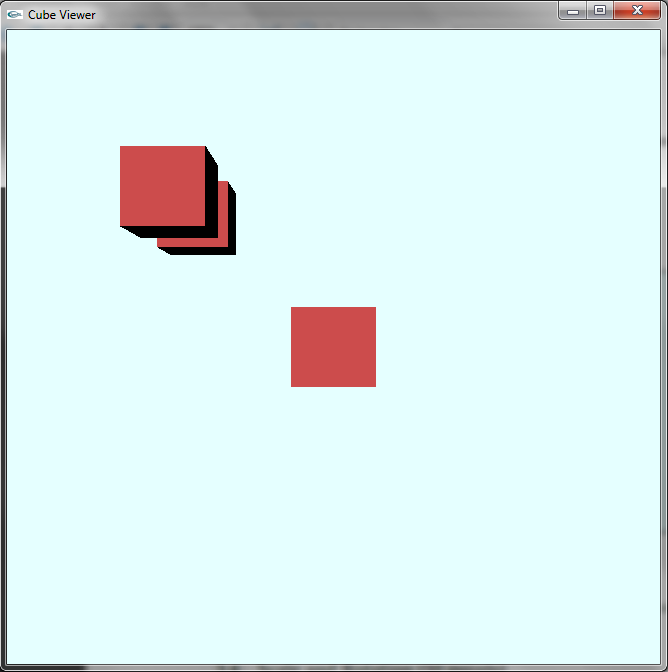
\includegraphics[width=0.5\textwidth]{3-3.png}
\end{figure}
\section*{3.4  Scale and Rotation}
The rotation matrix, given a angle and a axis, is given by (wikipedia)
\[ \left( \begin{array}{cccc}
cos(\theta)+u_x^2(1-cos(\theta)) & u_x u_y (1-cos(\theta))- u_z sin(\theta) & u_x u_z (1-cos(\theta))+ u_y \sin(theta) & 0\\
u_y u_x (1-cos(\theta)) + u_z sin(\theta) & cos(\theta)+u_y^2(1- cos(\theta)) & u_y u_z(1- cos(\theta)) - u_x sin(\theta) & 0\\
u_z u_x (1-cos(\theta)) -u_y sin(\theta) & u_z u_y (1-cos(\theta))+ u_y sin(\theta) & cos(\theta) + u_z^2(1-cos(\theta)) & 0\\
0 & 0 & 0 & 1\end{array} \right)\] 
where $u_x, u_y, u_z$ are component of the vector axis. Then $rotateWorld()$ and $rotateObject()$ are implemented in order like in part 3.2.

The scaling matrix is trivial and given in the course:
\[ \left( \begin{array}{cccc}
s & 0 & 0 & 0\\
0 & s & 0 & 0\\
0 & 0 & s & 0\\
0 & 0 & 0 & 1\end{array} \right)\] 

where $s$ is the scale.
Like before the function $scaleObject()$ and $scaleWorld()$ are implemented like 3.2.
\begin{figure}[h!]
\caption{Renderer the rotation and scaling}
  \centering
    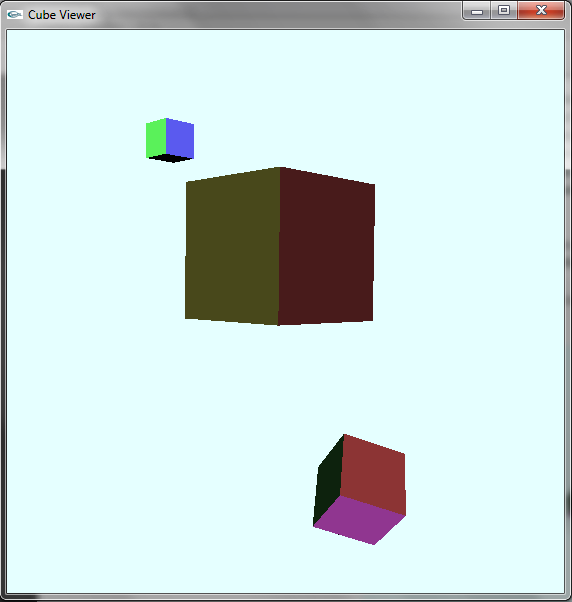
\includegraphics[width=0.5\textwidth]{3-4.png}
\end{figure}
\newpage
\section*{3.5 Clipping Planes}
If we cut the cube, we will have triangles, squares, pentagon and hexagon.
In this figure there are the cut we founded.
\begin{figure}[h!]
\caption{Shapes}
  \centering
    \includegraphics[width=0.5\textwidth]{formes.png}
\end{figure}
\end{document}